\documentclass{article}

% if you need to pass options to natbib, use, e.g.:
%     \PassOptionsToPackage{numbers, compress}{natbib}
% before loading neurips_2025

% The authors should use one of these tracks.
% Before accepting by the NeurIPS conference, select one of the options below.
% 0. "default" for submission
% \usepackage{neurips_2025}
% the "default" option is equal to the "main" option, which is used for the Main Track with double-blind reviewing.
% 1. "main" option is used for the Main Track
% \usepackage[main]{neurips_2025}
% 2. "position" option is used for the Position Paper Track
%  \usepackage[position]{neurips_2025}
% 3. "dandb" option is used for the Datasets & Benchmarks Track
% \usepackage[dandb]{neurips_2025}
% 4. "creativeai" option is used for the Creative AI Track
 \usepackage[creativeai]{neurips_2025}
% 5. "sglblindworkshop" option is used for the Workshop with single-blind reviewing
 % \usepackage[sglblindworkshop]{neurips_2025}
% 6. "dblblindworkshop" option is used for the Workshop with double-blind reviewing
%  \usepackage[dblblindworkshop]{neurips_2025}

% After being accepted, the authors should add "final" behind the track to compile a camera-ready version.
% 1. Main Track
% \usepackage[main, final]{neurips_2025}
% 2. Position Paper Track
%  \usepackage[position, final]{neurips_2025}
% 3. Datasets & Benchmarks Track
 % \usepackage[dandb, final]{neurips_2025}
% 4. Creative AI Track
%  \usepackage[creativeai, final]{neurips_2025}
% 5. Workshop with single-blind reviewing
%  \usepackage[sglblindworkshop, final]{neurips_2025}
% 6. Workshop with double-blind reviewing
%  \usepackage[dblblindworkshop, final]{neurips_2025}
% Note. For the workshop paper template, both \title{} and \workshoptitle{} are required, with the former indicating the paper title shown in the title and the latter indicating the workshop title displayed in the footnote.
% For workshops (5., 6.), the authors should add the name of the workshop, "\workshoptitle" command is used to set the workshop title.
% \workshoptitle{WORKSHOP TITLE}

% "preprint" option is used for arXiv or other preprint submissions
% \usepackage[preprint]{neurips_2025}

% to avoid loading the natbib package, add option nonatbib:
%\usepackage[nonatbib]{neurips_2025}
\usepackage[utf8]{inputenc} % allow utf-8 input
\usepackage[T1]{fontenc}    % use 8-bit T1 fonts
\usepackage{hyperref}       % hyperlinks
\usepackage{url}            % simple URL typesetting
\usepackage{booktabs}       % professional-quality tables
\usepackage{amsfonts}       % blackboard math symbols
\usepackage{nicefrac}       % compact symbols for 1/2, etc.
\usepackage{microtype}      % microtypography
\usepackage{xcolor}         % colors
\usepackage{tikz}           % diagrams
\usepackage{enumitem}       % customized lists
\usepackage{natbib}
\usetikzlibrary{arrows.meta,shapes,positioning,fit,backgrounds,calc}

% Note. For the workshop paper template, both \title{} and \workshoptitle{} are required, with the former indicating the paper title shown in the title and the latter indicating the workshop title displayed in the footnote. 
\title{Simulated Profiling Environment for Embodied I\underline{n}telligence (SPEEN)}


% The \author macro works with any number of authors. There are two commands
% used to separate the names and addresses of multiple authors: \And and \AND.
%
% Using \And between authors leaves it to LaTeX to determine where to break the
% lines. Using \AND forces a line break at that point. So, if LaTeX puts 3 of 4
% authors names on the first line, and the last on the second line, try using
% \AND instead of \And before the third author name.

\author{%
    Darroll Saddi\textsuperscript{1} \quad
        Ken Lin\textsuperscript{1} \quad
        Ryan Li\textsuperscript{1} \quad
        Matthew Fulde\textsuperscript{2} \quad
        Jon Lagasca\textsuperscript{1} \vspace{0.75em} \\
        \large{\textit{University of California, Davis}} \\
        \vspace{0.5em}
        \textsuperscript{1}Computer Science \quad
        \textsuperscript{2}Computer Science and Engineering \\
        \texttt{\{dwsaddi, kemlin, ryjli, mpfulde, jonlagasca\}@ucdavis.edu}
    }

\begin{document}

\maketitle

\begin{abstract}
    The Simulated Profiling Environment for Embodied Intelligence (SPEEN) is an open-source platform for evaluating embodied Large Language Model agents in a simulated game environment.
    As LLMs are increasingly integrated into robotics and embodied systems, SPEEN addresses the need for standardized evaluation frameworks by providing a modifiable system for benchmarking and implementing embodied LLM simulations in Godot.
    We implement a proof-of-concept Minecraft-like environment to demonstrate an application of this system, providing a structured quantitative benchmarking through diverse scenarios and an open-world sandbox for more qualitative assessment of decision-making behaviors.
    Our approach enables researchers and enthusiasts to test various embodied LLM implementations in a flexible simulated environment.
\end{abstract}

\section{Problem Identification}

\paragraph{Background}
This project originated as a Senior Design Project at UC Davis in collaboration with Justin Jia (affiliated with Apple) to address practical needs in AI testing.
The overarching goal of the project at this stage was to develop a sandbox environment specifically for testing AI programs.

\subsection{Exploratory Research}

\paragraph{Definitions}
We define agentic AI as systems capable of autonomous decision-making and environmental interaction, with embodied AI specifically concerning agents that interact with physical or simulated worlds.

\subsubsection{Focusing on Large Language Models}
Our research identified significant gaps in environmental design for evaluating advanced AI systems.
We examined existing platforms like NeuralMMO, which provides an open-source environment for measuring \textbf{reinforcement learning} algorithm performance in a 2D grid world with complex tasks that emulate a massively multiplayer online game.
A key insight from NeuralMMO's creator Joseph Suarez influenced our approach:
\begin{quote}
    "It is very easy to create an interesting looking simulator. It is very hard, under the constraints of making useful AI research [to create an environment meant for testing and training AI]…it is not just a game, it is an AI simulation."\footnote{Suarez, J. (2024, May 14). Joseph Suarez Thesis Defense - Neural MMO. YouTube. \url{https://www.youtube.com/watch?v=wwTOFYgtAWg}.}
\end{quote}
Furthermore, despite increasing environmental complexity, advanced algorithms like PPO were observed to be able to effectively solve most tasks given sufficient computation.
This shifted our focus away from reinforcement learning and toward Large Language Models, which have shown recent promise in integration with robotics and embodied systems.

\subsubsection{Environment Design}
There are a number of proposed embodied LLM architectures that use Minecraft as a testing environment.
Projects including NVIDIA's Voyager project (extending from the MineDojo project) and Project Sid by Altera\footnote{AL, A., Ahn, A., Becker, N., Carroll, S., Christie, N., Cortes, M., Demirci, A., Du, M., Li, F., Luo, S., Wang, P. Y., Willows, M., Yang, F., \& Yang, G. R. (2024). Project Sid: Many-agent simulations toward AI civilization. \url{https://arxiv.org/abs/2411.00114}.} attempt to provide prompting and training architectures for agents to exist in the game.
However, between these projects, there are identifiable limitationms as benchmarks of agentic LLMs:
\begin{itemize}
    \item \textbf{Lack of Open-Source Availability:}
          Project Sid articulates a way for many-agents to exist within Minecraft, proposing supposedly powerful prompting architectures, but is not open-source.
          It is further unclear how to reproduce the results from their methodology, representing potential conflict of interest
    \item \textbf{Limited Flexibility:}
          While MiniDojo projects like NVIDIA's Voyager\footnote{Wang, G., Xie, Y., Jiang, Y., Mandlekar, A., Xiao, C., Zhu, Y., Fan, L., \& Anandkumar, A. (2023). Voyager: An Open-Ended Embodied Agent with Large Language Models. \url{https://doi.org/10.48550/arXiv.2305.16291}.} have yielded impressive results and are open-source, we believe there is an increasing need to develop benchmarks that generalize to real-world use cases and to metrics specific to agentic AI rather than Minecraft.
          The domain-specific metrics of area explored \& percentage of available items collected are not necessarily useful for evaluating LLMs in a more general sense.
\end{itemize}

Additional barriers exist in the choice of environment.
While Minecraft offers inherent complexity and extensive documentation that may aid in implementation of the agents, it presents significant limitations as a benchmark:
\begin{enumerate}
    \item It requires a commercial license, creating accessibility barriers
    \item No existing standardized context provisioning or testing metrics
\end{enumerate}

\paragraph{Chosen Environment} Although environments that more closely emulate the real world would better map to real-world robotic applications, we determined that focusing on standardizing an accessible contextualization and prompting systems would be more beneficial for the field.
Thus, our focus was on the development of the prompting architecture, i.e. the interaction between the LLM and the game environment, and the collection of evaluation metrics, as opposed to purely on the environment itself.
With this in mind, our environment is kept less realistic and still similar to Minecraft, but we hope that future work will be able to build upon our work and expand to more realistic environments.

\subsubsection{Open-Source}
Our research identified that many successful LLM evaluation solutions are not open-source, limiting their utility for broader research purposes.
By building our system to allow for transparent and reproducible integration of new LLMs and prompting architectures, we aim to address this limitation.
This constraint guided our decision to use the Godot game engine, which is open-source and allows for easy modification and expansion.
Our selection of Godot was also motivated by its rapid development trajectory and growing community support, with major improvements in each release enhancing both performance and development workflows, showing great promise for use beyond simply game development.

\subsubsection{Research Use Case}
Ensuring our backend Python web socket supports both cloud-hosted and locally-hosted LLMs is important because this allows researchers to test various models as they're released.
Using abstraction layers, new models can be integrated into the system without requiring significant changes to the code base on the development side.
We implemented several different scenarios that stress test our API and agents capabilities for planning, environmental reasoning, and cooperation.
In the current product, we support the OpenAI GPT models, Google Gemini API, locally-hosted LLMs via OLlamma (Gemma3, Deepseek-r1, etc.).

\answerTODO{Mention Google Deepmind Creating Multimodal Interactive Agents with Imitation and Self-Supervised Learning }

\subsection{Design Requirements}
Based on our research findings, we had the sufficient justification to develop SPEEN as an open-source benchmarking environment specifically for evaluating embodied AI (LLM) performance.
Listed below were our comprehensive design goals and requirements for the system:
\begin{enumerate}
    \item \textbf{Standardized Evaluation Framework:}
          \begin{itemize}
              \item Quantitative metrics and qualitative assessment for embodied LLM agents
              \item Standardized prompting and game state context provisioning
              \item Streamlined integration of LLMs, prompting architectures, and evaluation methods
          \end{itemize}
    \item \textbf{LLM Integration Capabilities:}
          \begin{itemize}
              \item Support for cloud and locally-hosted LLMs
              \item Abstraction layers for seamless integration of any LLM
              \item High-level configuration options
          \end{itemize}
    \item \textbf{Open-Source Compliance:}
          \begin{itemize}
              \item Accessible and modifiable system with appropriate licensing for researchers and enthusiasts
              \item Comprehensive documentation
          \end{itemize}
\end{enumerate}
These are the requirements of the system we plan to achieve.
To prove its usability, we shall also implement the testing environment and prompting architecture as a proof of concept.
\begin{enumerate}
    \item \textbf{Accessible Game Environment:} A Minecraft-like 3D environment in Godot with sufficient complexity and intuitive interfaces for human researchers to monitor and evaluate agent performance
    \item \textbf{Structured Scenarios:} Diverse testing scenarios with automated performance scoring
    \item \textbf{Prompting Architecture:} Implement a prompting architecture emulating chain-of-thought and goal-based prompting systems with support for easy modification
\end{enumerate}

\section{Development}
\subsection{Environment Design}
A majority of early development focused on creating the agent's environment for qualitative evaluation.
Features included:
\begin{itemize}
    \item Procedural world generation with day/night cycle
    \item Navigation and A* pathfinding via Godot's Navigation3D system
    \item Suite of API functions for agent-environment interaction
    \item NPC AI (animals, zombies) for objectives and adversaries
    \item Item and inventory system
\end{itemize}
After around 7 weeks, we had a functional environment sufficiently complex for our proof of concept.

\subsection{Agent-Environment Pipeline}

\begin{figure}[ht!]
    \centering

    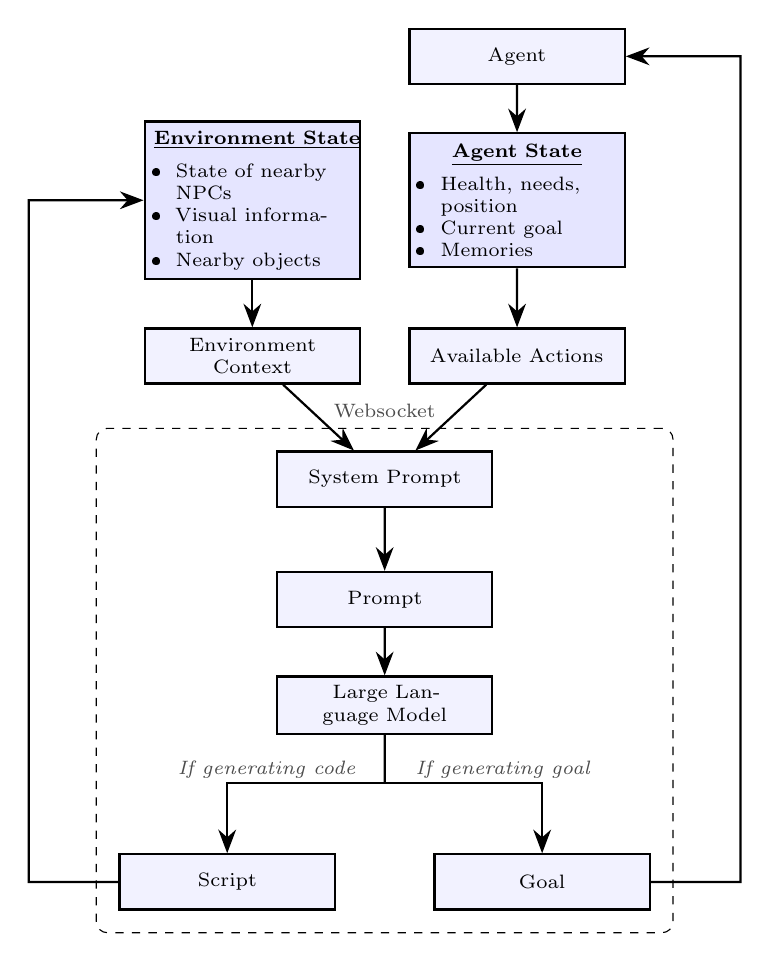
\begin{tikzpicture}[
        scale=0.18,
        node distance=0.6cm,
        box/.style={
                rectangle,
                draw,
                thick,
                minimum width=2cm,
                minimum height=1.7cm,
                text width=2.5cm,
                align=center,
                fill=blue!10,
                font=\scriptsize,
            },
        smallbox/.style={
                rectangle,
                draw,
                thick,
                minimum width=2cm,
                minimum height=0.7cm,
                text width=2.5cm,
                align=center,
                fill=blue!5,
                font=\scriptsize,
            },
        arrow/.style={-{Stealth[length=3mm]}, thick},
        condition/.style={font=\scriptsize\itshape, text opacity=0.7},
        ]
        % Define main component layer
        \node[box] (env) {\textbf{\underline{Environment State}} \\
            \begin{itemize}[leftmargin=1em, itemsep=0pt, topsep=2pt, parsep=0pt]
                \item State of nearby NPCs
                \item Visual information
                \item Nearby objects
            \end{itemize}};

        \node[box, right=of env] (agent_state) {\textbf{\underline{Agent State}} \\
            \begin{itemize}[leftmargin=1em, itemsep=0pt, topsep=2pt, parsep=0pt]
                \item Health, needs, position
                \item Current goal
                \item Memories
            \end{itemize}};

        \node[smallbox, above=of agent_state] (agent) {Agent};

        % Context processing layer - all on the same layer
        \node[smallbox, below=of env] (env_context) {Environment Context};
        \node[smallbox, right=of env_context] (actions) {Available Actions};

        % Calculate midpoint position for system prompt - now below env_context and actions
        \path (env_context) -- (actions) coordinate[midway] (mid_point);
        \node[smallbox, below=1.2cm of mid_point] (system_prompt) {System Prompt};

        % Prompt layer - moved down
        \node[smallbox, below=0.8cm of system_prompt] (prompt) {Prompt};

        % Connect system prompt to prompt
        \draw[arrow] (system_prompt) -- (prompt);

        % LLM layer - moved down
        \node[smallbox, below=of prompt] (llm) {Large Language Model};

        % Output layer - centered below LLM with appropriate spacing
        \path (llm.south west) -- (llm.south east) coordinate[midway] (llm_bottom);
        \node[smallbox, below=1.5cm of llm, xshift=-2cm] (script) {Script};
        \node[smallbox, below=1.5cm of llm, xshift=2cm] (goal) {Goal};

        % Add websocket label
        \node[draw, dashed, rounded corners, fit=(prompt)(system_prompt)(llm)(script)(goal), inner sep=8pt] (websocket_box) {};
        \node[font=\scriptsize, text opacity=0.7, yshift=6pt] at (websocket_box.north) {Websocket};

        % Main connections
        \draw[arrow] (env) -- (env_context);
        \draw[arrow] (agent_state) -- (actions);
        \draw[arrow] (agent) -- (agent_state);
        \draw[arrow] (env_context) -- (system_prompt);
        \draw[arrow] (actions) -- (system_prompt);
        \draw[arrow] (prompt) -- (llm);

        % Output paths
        \draw[thick] (llm) -- ++(0,-5.5) coordinate (branch_point);
        \draw[arrow] (branch_point) -| (script);
        \draw[arrow] (branch_point) -| (goal);

        % Add labels for conditions
        \node[condition, below=0.2cm of llm, xshift=-1.5cm] {If generating code};
        \node[condition, below=0.2cm of llm, xshift=1.5cm] {If generating goal};

        % Modified feedback paths - now exiting left and right then going up
        \draw[arrow] (script) -- ++(-14,0) |- (env.west);
        \draw[arrow] (goal) -- ++(14,0) |- (agent.east);
    \end{tikzpicture}

    \caption{Agent-Environment Pipeline Architecture}
    \label{fig:agent-pipeline}
\end{figure}

Figure \ref{fig:agent-pipeline}, depicts our agent-environment pipeline architecture, which also serves as our prompting architecture.
Environmental information is fed directly into the LLM, which generates either a script or a goal if no goal is set for the agent.
The LLM will execute the generated script, the outcome of which may be logged in the "Memories" of the agent.
The memory system represents our attempt to implement chain-of-thought reasoning, a common technique for emulating LLM decision making, as future context include the agent's memories.

The available actions are the API function calls available to the agent, which abstract away the low-level interaction logic of the environment.
This technique focuses the LLM on reasoning and decision making rather than on code adherence, although it is possible for broken code to be generated.
In this event, we catch broken code and are able to either re-prompt with the error for self-fixing behavior, or alternatively count the iteration as a failure.

Once the script is ready to be ran, the agent's "body" will execute the input actions from the LLM till script completion.
The pipeline then repeats from the beginning and continues repeating until the scenario goal is satisfied or the specified max amount of iterations is reached.

\section{Testing and Evaluation}
\subsection{Benchmarking Scenarios}

We implemented a variety of scenarios to test different aspects of agent capabilities:
\begin{enumerate}
    \item Basic navigation: Testing the agent's ability to navigate to specific locations
    \item Item manipulation: Testing picking up and giving items
    \item Entity Interaction: Testing communication and combat with other entities
    \item Sequential Tasks: Testing the agent's ability to perform multi-step tasks
\end{enumerate}
Each scenario includes success criteria and automatic performance tracking.

\subsection{ Evaluation Metric}
The system tracks several key metrics:
\begin{itemize}
    \item Success Rate: Percentage of tasks completed successfully
    \item Failure Rate: Percentage of tasks that failed to complete
          \begin{itemize}
              \item Counting errors in code compilation and logical errors as failures
          \end{itemize}
\end{itemize}

\section{Connecting to Sandia Mission Areas and NAE Grand Challenges}
\subsection{Relevance to Sandia Mission Areas}
Our project aligns with several Sandia National Laboratories' mission areas:
\begin{enumerate}
    \item Computing and Information Sciences: SPEEN provides a platform for evaluating and improving computational intelligence systems, directly supporting Sandia's work in advanced computing and software engineering.
          Our system enables systematic testing of AI capabilities.
    \item National Security Technologies: By developing evaluation frameworks for embodied AI, we contribute to technologies that could enhance decision-making systems relevant to nation security applications.
          Autonomous AI systems require rigorous evaluation before deployment, which SPEEN facilitates
    \item Engineering Sciences: The design and implementation of our evaluation environment draws on principles from systems engineering, human-machine interfaces, and simulation technology, all core engineering areas within Sandia's scope of research
\end{enumerate}

\subsection{Connection to NAE Grand Challenges}
Our work addresses aspects of multiple National Academy of Engineering Grand Challenges
\begin{enumerate}
    \item Engineer the Tools of Scientific Discovery: SPEEN serves as a tool for scientific discovery in the field of artificial intelligence, allowing researchers to systematically evaluate and improve embodied AI systems.
          This directly supports NAE's challenge to develop better tools for scientific understanding
    \item Enhanced Virtual Reality: Our platform advances techniques for creating interactive, responsive virtual environments with intelligent agents.
          These environments can simulate and test what AI systems that could operate in the physical world.
    \item Advanced AI for Improved Quality of Life: By developing better evaluation methods for embodied AI, we contribute to the broader goal of creating AI systems that can effectively assist humans in daily life and critical operations.
          Reliable AI requires thorough testing like those we've developed.
\end{enumerate}

\section{Conclusion and future developments}
LLMs are a relatively new technology, meaning there are not many tools for measuring LLMs' competency in decision-making and environment interaction.
There are projects such as Mindcraft\footnote{kolbytn. (2023). GitHub - kolbytn/mindcraft. GitHub. \url{(https://github.com/kolbytn/mindcraft)}.} and Voyager that do integrate LLMs into a virtual world but lack benchmarking features for researchers to record their LLMs' performance and are built for Minecraft itself, requiring researchers to obtain paid licenses for Minecraft.
Our project aims to be the solution to the problems of benchmarking tools and accessibility.
With the ease of including new LLMs and the provided benchmarking scenarios, we hope to accelerate advancements in embodied AI systems involving LLMs.

\end{document}

% \newpage

% \section{Helpful formatting tools from Neurips}

% \paragraph{Paragraphs}

% There is also a \verb+\paragraph+ command available, which sets the heading in
% bold, flush left, and inline with the text, with the heading followed by 1\,em
% of space.

% If you wish to load the \verb+natbib+ package with options, you may add the
% following before loading the \verb+neurips_2025+ package:
% \begin{verbatim}
%    \PassOptionsToPackage{options}{natbib}
% \end{verbatim}

% If \verb+natbib+ clashes with another package you load, you can add the optional
% argument \verb+nonatbib+ when loading the style file:
% \begin{verbatim}
%    \usepackage[nonatbib]{neurips_2025}
% \end{verbatim}

% As submission is double blind, refer to your own published work in the third
% person. That is, use ``In the previous work of Jones et al.\ [4],'' not ``In our
% previous work [4].'' If you cite your other papers that are not widely available
% (e.g., a journal paper under review), use anonymous author names in the
% citation, e.g., an author of the form ``A.\ Anonymous'' and include a copy of the anonymized paper in the supplementary material.

% \subsection{Footnotes}

% Footnotes should be used sparingly.  If you do require a footnote, indicate
% footnotes with a number\footnote{Sample of the first footnote.} in the
% text. Place the footnotes at the bottom of the page on which they appear.
% Precede the footnote with a horizontal rule of 2~inches (12~picas).

% Note that footnotes are properly typeset \emph{after} punctuation
% marks.\footnote{As in this example.}

% \subsection{Figures}

% \begin{figure}
%     \centering
%     \fbox{\rule[-.5cm]{0cm}{4cm} \rule[-.5cm]{4cm within}{0cm}}
%     \caption{Sample figure caption.}
% \end{figure}

% All artwork must be neat, clean, and legible. Lines should be dark enough for
% purposes of reproduction. The figure number and caption always appear after the
% figure. Place one line space before the figure caption and one line space after
% the figure. The figure caption should be lower case (except for first word and
% proper nouns); figures are numbered consecutively.

% You may use color figures.  However, it is best for the figure captions and the
% paper body to be legible if the paper is printed in either black/white or in
% color.

% \subsection{Tables}

% All tables must be centered, neat, clean and legible.  The table number and
% title always appear before the table.  See Table~\ref{sample-table}.

% Place one line space before the table title, one line space after the
% table title, and one line space after the table. The table title must
% be lower case (except for first word and proper nouns); tables are
% numbered consecutively.

% Note that publication-quality tables \emph{do not contain vertical rules.} We
% strongly suggest the use of the \verb+booktabs+ package, which allows for
% typesetting high-quality, professional tables:
% \begin{center}
%     \url{https://www.ctan.org/pkg/booktabs}
% \end{center}
% This package was used to typeset Table~\ref{sample-table}.

% \begin{table}
%     \caption{Sample table title}
%     \label{sample-table}
%     \centering
%     \begin{tabular}{lll}
%         \toprule
%         \multicolumn{2}{c}{Part}                   \\
%         \cmidrule(r){1-2}
%         Name     & Description     & Size ($\mu$m) \\
%         \midrule
%         Dendrite & Input terminal  & $\sim$100     \\
%         Axon     & Output terminal & $\sim$10      \\
%         Soma     & Cell body       & up to $10^6$  \\
%         \bottomrule
%     \end{tabular}
% \end{table}

% \subsection{Math}
% Note that display math in bare TeX commands will not create correct line numbers for submission. Please use LaTeX (or AMSTeX) commands for unnumbered display math. (You really shouldn't be using \$\$ anyway; see \url{https://tex.stackexchange.com/questions/503/why-is-preferable-to} and \url{https://tex.stackexchange.com/questions/40492/what-are-the-differences-between-align-equation-and-displaymath} for more information.)

% \subsection{Final instructions}

% Do not change any aspects of the formatting parameters in the style files.  In
% particular, do not modify the width or length of the rectangle the text should
% fit into, and do not change font sizes (except perhaps in the
% \textbf{References} section; see below). Please note that pages should be
% numbered.

% \section*{References}


% References follow the acknowledgments in the camera-ready paper. Use unnumbered first-level heading for
% the references. Any choice of citation style is acceptable as long as you are
% consistent. It is permissible to reduce the font size to \verb+small+ (9 point)
% when listing the references.
% Note that the Reference section does not count towards the page limit.
% \medskip


% {
% \small


% [1] Alexander, J.A.\ \& Mozer, M.C.\ (1995) Template-based algorithms for
% connectionist rule extraction. In G.\ Tesauro, D.S.\ Touretzky and T.K.\ Leen
% (eds.), {\it Advances in Neural Information Processing Systems 7},
% pp.\ 609--616. Cambridge, MA: MIT Press.


%     [2] Bower, J.M.\ \& Beeman, D.\ (1995) {\it The Book of GENESIS: Exploring
%         Realistic Neural Models with the GEneral NEural SImulation System.}  New York:
% TELOS/Springer--Verlag.


% [3] Hasselmo, M.E., Schnell, E.\ \& Barkai, E.\ (1995) Dynamics of learning and
% recall at excitatory recurrent synapses and cholinergic modulation in rat
% hippocampal region CA3. {\it Journal of Neuroscience} {\bf 15}(7):5249-5262.
% }


% %%%%%%%%%%%%%%%%%%%%%%%%%%%%%%%%%%%%%%%%%%%%%%%%%%%%%%%%%%%%

% \appendix

% \section{Technical Appendices and Supplementary Material}
% Technical appendices with additional results, figures, graphs and proofs may be submitted with the paper submission before the full submission deadline (see above), or as a separate PDF in the ZIP file below before the supplementary material deadline. There is no page limit for the technical appendices.

% %%%%%%%%%%%%%%%%%%%%%%%%%%%%%%%%%%%%%%%%%%%%%%%%%%%%%%%%%%%%

% \newpage
% \section*{NeurIPS Paper Checklist}

% %%% BEGIN INSTRUCTIONS %%%
% The checklist is designed to encourage best practices for responsible machine learning research, addressing issues of reproducibility, transparency, research ethics, and societal impact. Do not remove the checklist: {\bf The papers not including the checklist will be desk rejected.} The checklist should follow the references and follow the (optional) supplemental material.  The checklist does NOT count towards the page
% limit.

% Please read the checklist guidelines carefully for information on how to answer these questions. For each question in the checklist:
% \begin{itemize}
%     \item You should answer \answerYes{}, \answerNo{}, or \answerNA{}.
%     \item \answerNA{} means either that the question is Not Applicable for that particular paper or the relevant information is Not Available.
%     \item Please provide a short (1–2 sentence) justification right after your answer (even for NA).
%           % \item {\bf The papers not including the checklist will be desk rejected.}
% \end{itemize}

% {\bf The checklist answers are an integral part of your paper submission.} They are visible to the reviewers, area chairs, senior area chairs, and ethics reviewers. You will be asked to also include it (after eventual revisions) with the final version of your paper, and its final version will be published with the paper.

% The reviewers of your paper will be asked to use the checklist as one of the factors in their evaluation. While "\answerYes{}" is generally preferable to "\answerNo{}", it is perfectly acceptable to answer "\answerNo{}" provided a proper justification is given (e.g., "error bars are not reported because it would be too computationally expensive" or "we were unable to find the license for the dataset we used"). In general, answering "\answerNo{}" or "\answerNA{}" is not grounds for rejection. While the questions are phrased in a binary way, we acknowledge that the true answer is often more nuanced, so please just use your best judgment and write a justification to elaborate. All supporting evidence can appear either in the main paper or the supplemental material, provided in appendix. If you answer \answerYes{} to a question, in the justification please point to the section(s) where related material for the question can be found.

% IMPORTANT, please:
% \begin{itemize}
%     \item {\bf Delete this instruction block, but keep the section heading ``NeurIPS Paper Checklist"},
%     \item  {\bf Keep the checklist subsection headings, questions/answers and guidelines below.}
%     \item {\bf Do not modify the questions and only use the provided macros for your answers}.
% \end{itemize}


% %%% END INSTRUCTIONS %%%


% \begin{enumerate}

%     \item {\bf Claims}
%     \item[] Question: Do the main claims made in the abstract and introduction accurately reflect the paper's contributions and scope?
%     \item[] Answer: \answerTODO{} % Replace by \answerYes{}, \answerNo{}, or \answerNA{}.
%     \item[] Justification: \justificationTODO{}
%     \item[] Guidelines:
%           \begin{itemize}
%               \item The answer NA means that the abstract and introduction do not include the claims made in the paper.
%               \item The abstract and/or introduction should clearly state the claims made, including the contributions made in the paper and important assumptions and limitations. A No or NA answer to this question will not be perceived well by the reviewers.
%               \item The claims made should match theoretical and experimental results, and reflect how much the results can be expected to generalize to other settings.
%               \item It is fine to include aspirational goals as motivation as long as it is clear that these goals are not attained by the paper.
%           \end{itemize}

%     \item {\bf Limitations}
%     \item[] Question: Does the paper discuss the limitations of the work performed by the authors?
%     \item[] Answer: \answerTODO{} % Replace by \answerYes{}, \answerNo{}, or \answerNA{}.
%     \item[] Justification: \justificationTODO{}
%     \item[] Guidelines:
%           \begin{itemize}
%               \item The answer NA means that the paper has no limitation while the answer No means that the paper has limitations, but those are not discussed in the paper.
%               \item The authors are encouraged to create a separate "Limitations" section in their paper.
%               \item The paper should point out any strong assumptions and how robust the results are to violations of these assumptions (e.g., independence assumptions, noiseless settings, model well-specification, asymptotic approximations only holding locally). The authors should reflect on how these assumptions might be violated in practice and what the implications would be.
%               \item The authors should reflect on the scope of the claims made, e.g., if the approach was only tested on a few datasets or with a few runs. In general, empirical results often depend on implicit assumptions, which should be articulated.
%               \item The authors should reflect on the factors that influence the performance of the approach. For example, a facial recognition algorithm may perform poorly when image resolution is low or images are taken in low lighting. Or a speech-to-text system might not be used reliably to provide closed captions for online lectures because it fails to handle technical jargon.
%               \item The authors should discuss the computational efficiency of the proposed algorithms and how they scale with dataset size.
%               \item If applicable, the authors should discuss possible limitations of their approach to address problems of privacy and fairness.
%               \item While the authors might fear that complete honesty about limitations might be used by reviewers as grounds for rejection, a worse outcome might be that reviewers discover limitations that aren't acknowledged in the paper. The authors should use their best judgment and recognize that individual actions in favor of transparency play an important role in developing norms that preserve the integrity of the community. Reviewers will be specifically instructed to not penalize honesty concerning limitations.
%           \end{itemize}

%     \item {\bf Theory assumptions and proofs}
%     \item[] Question: For each theoretical result, does the paper provide the full set of assumptions and a complete (and correct) proof?
%     \item[] Answer: \answerTODO{} % Replace by \answerYes{}, \answerNo{}, or \answerNA{}.
%     \item[] Justification: \justificationTODO{}
%     \item[] Guidelines:
%           \begin{itemize}
%               \item The answer NA means that the paper does not include theoretical results.
%               \item All the theorems, formulas, and proofs in the paper should be numbered and cross-referenced.
%               \item All assumptions should be clearly stated or referenced in the statement of any theorems.
%               \item The proofs can either appear in the main paper or the supplemental material, but if they appear in the supplemental material, the authors are encouraged to provide a short proof sketch to provide intuition.
%               \item Inversely, any informal proof provided in the core of the paper should be complemented by formal proofs provided in appendix or supplemental material.
%               \item Theorems and Lemmas that the proof relies upon should be properly referenced.
%           \end{itemize}

%     \item {\bf Experimental result reproducibility}
%     \item[] Question: Does the paper fully disclose all the information needed to reproduce the main experimental results of the paper to the extent that it affects the main claims and/or conclusions of the paper (regardless of whether the code and data are provided or not)?
%     \item[] Answer: \answerTODO{} % Replace by \answerYes{}, \answerNo{}, or \answerNA{}.
%     \item[] Justification: \justificationTODO{}
%     \item[] Guidelines:
%           \begin{itemize}
%               \item The answer NA means that the paper does not include experiments.
%               \item If the paper includes experiments, a No answer to this question will not be perceived well by the reviewers: Making the paper reproducible is important, regardless of whether the code and data are provided or not.
%               \item If the contribution is a dataset and/or model, the authors should describe the steps taken to make their results reproducible or verifiable.
%               \item Depending on the contribution, reproducibility can be accomplished in various ways. For example, if the contribution is a novel architecture, describing the architecture fully might suffice, or if the contribution is a specific model and empirical evaluation, it may be necessary to either make it possible for others to replicate the model with the same dataset, or provide access to the model. In general. releasing code and data is often one good way to accomplish this, but reproducibility can also be provided via detailed instructions for how to replicate the results, access to a hosted model (e.g., in the case of a large language model), releasing of a model checkpoint, or other means that are appropriate to the research performed.
%               \item While NeurIPS does not require releasing code, the conference does require all submissions to provide some reasonable avenue for reproducibility, which may depend on the nature of the contribution. For example
%                     \begin{enumerate}
%                         \item If the contribution is primarily a new algorithm, the paper should make it clear how to reproduce that algorithm.
%                         \item If the contribution is primarily a new model architecture, the paper should describe the architecture clearly and fully.
%                         \item If the contribution is a new model (e.g., a large language model), then there should either be a way to access this model for reproducing the results or a way to reproduce the model (e.g., with an open-source dataset or instructions for how to construct the dataset).
%                         \item We recognize that reproducibility may be tricky in some cases, in which case authors are welcome to describe the particular way they provide for reproducibility. In the case of closed-source models, it may be that access to the model is limited in some way (e.g., to registered users), but it should be possible for other researchers to have some path to reproducing or verifying the results.
%                     \end{enumerate}
%           \end{itemize}


%     \item {\bf Open access to data and code}
%     \item[] Question: Does the paper provide open access to the data and code, with sufficient instructions to faithfully reproduce the main experimental results, as described in supplemental material?
%     \item[] Answer: \answerTODO{} % Replace by \answerYes{}, \answerNo{}, or \answerNA{}.
%     \item[] Justification: \justificationTODO{}
%     \item[] Guidelines:
%           \begin{itemize}
%               \item The answer NA means that paper does not include experiments requiring code.
%               \item Please see the NeurIPS code and data submission guidelines (\url{https://nips.cc/public/guides/CodeSubmissionPolicy}) for more details.
%               \item While we encourage the release of code and data, we understand that this might not be possible, so “No” is an acceptable answer. Papers cannot be rejected simply for not including code, unless this is central to the contribution (e.g., for a new open-source benchmark).
%               \item The instructions should contain the exact command and environment needed to run to reproduce the results. See the NeurIPS code and data submission guidelines (\url{https://nips.cc/public/guides/CodeSubmissionPolicy}) for more details.
%               \item The authors should provide instructions on data access and preparation, including how to access the raw data, preprocessed data, intermediate data, and generated data, etc.
%               \item The authors should provide scripts to reproduce all experimental results for the new proposed method and baselines. If only a subset of experiments are reproducible, they should state which ones are omitted from the script and why.
%               \item At submission time, to preserve anonymity, the authors should release anonymized versions (if applicable).
%               \item Providing as much information as possible in supplemental material (appended to the paper) is recommended, but including URLs to data and code is permitted.
%           \end{itemize}


%     \item {\bf Experimental setting/details}
%     \item[] Question: Does the paper specify all the training and test details (e.g., data splits, hyperparameters, how they were chosen, type of optimizer, etc.) necessary to understand the results?
%     \item[] Answer: \answerTODO{} % Replace by \answerYes{}, \answerNo{}, or \answerNA{}.
%     \item[] Justification: \justificationTODO{}
%     \item[] Guidelines:
%           \begin{itemize}
%               \item The answer NA means that the paper does not include experiments.
%               \item The experimental setting should be presented in the core of the paper to a level of detail that is necessary to appreciate the results and make sense of them.
%               \item The full details can be provided either with the code, in appendix, or as supplemental material.
%           \end{itemize}

%     \item {\bf Experiment statistical significance}
%     \item[] Question: Does the paper report error bars suitably and correctly defined or other appropriate information about the statistical significance of the experiments?
%     \item[] Answer: \answerTODO{} % Replace by \answerYes{}, \answerNo{}, or \answerNA{}.
%     \item[] Justification: \justificationTODO{}
%     \item[] Guidelines:
%           \begin{itemize}
%               \item The answer NA means that the paper does not include experiments.
%               \item The authors should answer "Yes" if the results are accompanied by error bars, confidence intervals, or statistical significance tests, at least for the experiments that support the main claims of the paper.
%               \item The factors of variability that the error bars are capturing should be clearly stated (for example, train/test split, initialization, random drawing of some parameter, or overall run with given experimental conditions).
%               \item The method for calculating the error bars should be explained (closed form formula, call to a library function, bootstrap, etc.)
%               \item The assumptions made should be given (e.g., Normally distributed errors).
%               \item It should be clear whether the error bar is the standard deviation or the standard error of the mean.
%               \item It is OK to report 1-sigma error bars, but one should state it. The authors should preferably report a 2-sigma error bar than state that they have a 96\% CI, if the hypothesis of Normality of errors is not verified.
%               \item For asymmetric distributions, the authors should be careful not to show in tables or figures symmetric error bars that would yield results that are out of range (e.g. negative error rates).
%               \item If error bars are reported in tables or plots, The authors should explain in the text how they were calculated and reference the corresponding figures or tables in the text.
%           \end{itemize}

%     \item {\bf Experiments compute resources}
%     \item[] Question: For each experiment, does the paper provide sufficient information on the computer resources (type of compute workers, memory, time of execution) needed to reproduce the experiments?
%     \item[] Answer: \answerTODO{} % Replace by \answerYes{}, \answerNo{}, or \answerNA{}.
%     \item[] Justification: \justificationTODO{}
%     \item[] Guidelines:
%           \begin{itemize}
%               \item The answer NA means that the paper does not include experiments.
%               \item The paper should indicate the type of compute workers CPU or GPU, internal cluster, or cloud provider, including relevant memory and storage.
%               \item The paper should provide the amount of compute required for each of the individual experimental runs as well as estimate the total compute.
%               \item The paper should disclose whether the full research project required more compute than the experiments reported in the paper (e.g., preliminary or failed experiments that didn't make it into the paper).
%           \end{itemize}

%     \item {\bf Code of ethics}
%     \item[] Question: Does the research conducted in the paper conform, in every respect, with the NeurIPS Code of Ethics \url{https://neurips.cc/public/EthicsGuidelines}?
%     \item[] Answer: \answerTODO{} % Replace by \answerYes{}, \answerNo{}, or \answerNA{}.
%     \item[] Justification: \justificationTODO{}
%     \item[] Guidelines:
%           \begin{itemize}
%               \item The answer NA means that the authors have not reviewed the NeurIPS Code of Ethics.
%               \item If the authors answer No, they should explain the special circumstances that require a deviation from the Code of Ethics.
%               \item The authors should make sure to preserve anonymity (e.g., if there is a special consideration due to laws or regulations in their jurisdiction).
%           \end{itemize}


%     \item {\bf Broader impacts}
%     \item[] Question: Does the paper discuss both potential positive societal impacts and negative societal impacts of the work performed?
%     \item[] Answer: \answerTODO{} % Replace by \answerYes{}, \answerNo{}, or \answerNA{}.
%     \item[] Justification: \justificationTODO{}
%     \item[] Guidelines:
%           \begin{itemize}
%               \item The answer NA means that there is no societal impact of the work performed.
%               \item If the authors answer NA or No, they should explain why their work has no societal impact or why the paper does not address societal impact.
%               \item Examples of negative societal impacts include potential malicious or unintended uses (e.g., disinformation, generating fake profiles, surveillance), fairness considerations (e.g., deployment of technologies that could make decisions that unfairly impact specific groups), privacy considerations, and security considerations.
%               \item The conference expects that many papers will be foundational research and not tied to particular applications, let alone deployments. However, if there is a direct path to any negative applications, the authors should point it out. For example, it is legitimate to point out that an improvement in the quality of generative models could be used to generate deepfakes for disinformation. On the other hand, it is not needed to point out that a generic algorithm for optimizing neural networks could enable people to train models that generate Deepfakes faster.
%               \item The authors should consider possible harms that could arise when the technology is being used as intended and functioning correctly, harms that could arise when the technology is being used as intended but gives incorrect results, and harms following from (intentional or unintentional) misuse of the technology.
%               \item If there are negative societal impacts, the authors could also discuss possible mitigation strategies (e.g., gated release of models, providing defenses in addition to attacks, mechanisms for monitoring misuse, mechanisms to monitor how a system learns from feedback over time, improving the efficiency and accessibility of ML).
%           \end{itemize}

%     \item {\bf Safeguards}
%     \item[] Question: Does the paper describe safeguards that have been put in place for responsible release of data or models that have a high risk for misuse (e.g., pretrained language models, image generators, or scraped datasets)?
%     \item[] Answer: \answerTODO{} % Replace by \answerYes{}, \answerNo{}, or \answerNA{}.
%     \item[] Justification: \justificationTODO{}
%     \item[] Guidelines:
%           \begin{itemize}
%               \item The answer NA means that the paper poses no such risks.
%               \item Released models that have a high risk for misuse or dual-use should be released with necessary safeguards to allow for controlled use of the model, for example by requiring that users adhere to usage guidelines or restrictions to access the model or implementing safety filters.
%               \item Datasets that have been scraped from the Internet could pose safety risks. The authors should describe how they avoided releasing unsafe images.
%               \item We recognize that providing effective safeguards is challenging, and many papers do not require this, but we encourage authors to take this into account and make a best faith effort.
%           \end{itemize}

%     \item {\bf Licenses for existing assets}
%     \item[] Question: Are the creators or original owners of assets (e.g., code, data, models), used in the paper, properly credited and are the license and terms of use explicitly mentioned and properly respected?
%     \item[] Answer: \answerTODO{} % Replace by \answerYes{}, \answerNo{}, or \answerNA{}.
%     \item[] Justification: \justificationTODO{}
%     \item[] Guidelines:
%           \begin{itemize}
%               \item The answer NA means that the paper does not use existing assets.
%               \item The authors should cite the original paper that produced the code package or dataset.
%               \item The authors should state which version of the asset is used and, if possible, include a URL.
%               \item The name of the license (e.g., CC-BY 4.0) should be included for each asset.
%               \item For scraped data from a particular source (e.g., website), the copyright and terms of service of that source should be provided.
%               \item If assets are released, the license, copyright information, and terms of use in the package should be provided. For popular datasets, \url{paperswithcode.com/datasets} has curated licenses for some datasets. Their licensing guide can help determine the license of a dataset.
%               \item For existing datasets that are re-packaged, both the original license and the license of the derived asset (if it has changed) should be provided.
%               \item If this information is not available online, the authors are encouraged to reach out to the asset's creators.
%           \end{itemize}

%     \item {\bf New assets}
%     \item[] Question: Are new assets introduced in the paper well documented and is the documentation provided alongside the assets?
%     \item[] Answer: \answerTODO{} % Replace by \answerYes{}, \answerNo{}, or \answerNA{}.
%     \item[] Justification: \justificationTODO{}
%     \item[] Guidelines:
%           \begin{itemize}
%               \item The answer NA means that the paper does not release new assets.
%               \item Researchers should communicate the details of the dataset/code/model as part of their submissions via structured templates. This includes details about training, license, limitations, etc.
%               \item The paper should discuss whether and how consent was obtained from people whose asset is used.
%               \item At submission time, remember to anonymize your assets (if applicable). You can either create an anonymized URL or include an anonymized zip file.
%           \end{itemize}

%     \item {\bf Crowdsourcing and research with human subjects}
%     \item[] Question: For crowdsourcing experiments and research with human subjects, does the paper include the full text of instructions given to participants and screenshots, if applicable, as well as details about compensation (if any)?
%     \item[] Answer: \answerTODO{} % Replace by \answerYes{}, \answerNo{}, or \answerNA{}.
%     \item[] Justification: \justificationTODO{}
%     \item[] Guidelines:
%           \begin{itemize}
%               \item The answer NA means that the paper does not involve crowdsourcing nor research with human subjects.
%               \item Including this information in the supplemental material is fine, but if the main contribution of the paper involves human subjects, then as much detail as possible should be included in the main paper.
%               \item According to the NeurIPS Code of Ethics, workers involved in data collection, curation, or other labor should be paid at least the minimum wage in the country of the data collector.
%           \end{itemize}

%     \item {\bf Institutional review board (IRB) approvals or equivalent for research with human subjects}
%     \item[] Question: Does the paper describe potential risks incurred by study participants, whether such risks were disclosed to the subjects, and whether Institutional Review Board (IRB) approvals (or an equivalent approval/review based on the requirements of your country or institution) were obtained?
%     \item[] Answer: \answerTODO{} % Replace by \answerYes{}, \answerNo{}, or \answerNA{}.
%     \item[] Justification: \justificationTODO{}
%     \item[] Guidelines:
%           \begin{itemize}
%               \item The answer NA means that the paper does not involve crowdsourcing nor research with human subjects.
%               \item Depending on the country in which research is conducted, IRB approval (or equivalent) may be required for any human subjects research. If you obtained IRB approval, you should clearly state this in the paper.
%               \item We recognize that the procedures for this may vary significantly between institutions and locations, and we expect authors to adhere to the NeurIPS Code of Ethics and the guidelines for their institution.
%               \item For initial submissions, do not include any information that would break anonymity (if applicable), such as the institution conducting the review.
%           \end{itemize}

%     \item {\bf Declaration of LLM usage}
%     \item[] Question: Does the paper describe the usage of LLMs if it is an important, original, or non-standard component of the core methods in this research? Note that if the LLM is used only for writing, editing, or formatting purposes and does not impact the core methodology, scientific rigorousness, or originality of the research, declaration is not required.
%           %this research? 
%     \item[] Answer: \answerTODO{} % Replace by \answerYes{}, \answerNo{}, or \answerNA{}.
%     \item[] Justification: \justificationTODO{}
%     \item[] Guidelines:
%           \begin{itemize}
%               \item The answer NA means that the core method development in this research does not involve LLMs as any important, original, or non-standard components.
%               \item Please refer to our LLM policy (\url{https://neurips.cc/Conferences/2025/LLM}) for what should or should not be described.
%           \end{itemize}

% \end{enumerate}


\end{document}